\documentclass[fleqn, usenatbib, useAMS, a4paper]{mnras}
\usepackage{graphicx}
\usepackage{amsmath,paralist,xcolor,xspace,amssymb}
\usepackage{times}
\usepackage{comment}

\newcommand{\gadget}{{\sc Gadget}\xspace}
\newcommand{\swift}{{\sc Swift}\xspace}
\newcommand{\nbody}{$N$-body\xspace}

%opening
\title{FMM in SWIFT}
\author{Matthieu Schaller}
\begin{document}

\date{\today}

\pagerange{\pageref{firstpage}--\pageref{lastpage}} \pubyear{2014}

\maketitle

\label{firstpage}

\begin{abstract}
\end{abstract}

\begin{keywords}
\end{keywords}

\section{Gravity in \swift}
\label{sec:gravity}

\subsection{Gravitational softening}
\label{ssec:potential_softening}

To avoid artificial two-body relaxation, the Dirac
$\delta$-distribution corresponding to each particle is convolved with
a softening kernel of a given fixed, but time-variable, scale-length
$H$. Instead of the commonly used spline kernel of
\cite{Monaghan1985} (e.g. in \textsc{Gadget}), we use a C2 kernel
\citep{Wendland1995} which leads to an expression for the force that
is cheaper to compute and has a very similar overall shape. The C2
kernel has the advantage of being branch-free leading to an expression
which is faster to evaluate using vector units available on modern
architectures; it also does not require any divisions to evaluate the
softened forces. We set $\tilde\delta(\mathbf{r}) = \rho(|\mathbf{r}|)
= W(|\mathbf{r}|, 3\epsilon_{\rm Plummer})$, with $W(r, H)$ given by

\begin{align}
W(r,H) &= \frac{21}{2\pi H^3} \times \nonumber \\
&\left\lbrace\begin{array}{rcl}
4u^5 - 15u^4 + 20u^3 - 10u^2 + 1 & \mbox{if} & u < 1,\\
0 & \mbox{if} & u \geq 1,
\end{array}
\right.
\end{align}
and $u = r/H$. The potential $\varphi(r,H)$ corresponding to this density distribution reads
\begin{align}
\varphi(r,H) = 
\left\lbrace\begin{array}{rcl}
f(\frac{r}{H}) \times H^{-1} & \mbox{if} & r < H,\\
r^{-1} & \mbox{if} & r \geq H,
\end{array}
\right.
\label{eq:fmm:potential}
\end{align}
with $f(u) \equiv -3u^7 + 15u^6 - 28u^5 + 21u^4 - 7u^2 + 3$. These
choices lead to a potential at $|\mathbf{x}| = 0$ equal to the central
potential of a Plummer sphere (i.e. $\varphi(0) = 1/\epsilon_{\rm
  Plummer}$)\footnote{Note the factor $3$ in the definition of
  $\rho(|\mathbf{x}|)$ which differs from the factor $2.8$ used for
  the cubic spline kernel as a consequence of the change of the functional
  form of $W$.}. From this expression the softened gravitational force can
be easily obtained:
\begin{align}
\mathbf{\nabla}\varphi(r,H) = \mathbf{r} \cdot
\left\lbrace\begin{array}{rcl}
g(\frac{r}{H}) \times H^{-3} & \mbox{if} & r < H,\\
r^{-3} & \mbox{if} & r \geq H,
\end{array}
\right.
\label{eq:fmm:force}
\end{align}
with $g(u) \equiv f'(u)/u = -21u^5+90u^4-140u^3+84u^2-14$. This last
expression has the advantage of not containing any divisions or
branching (besides the always necessary check for $r<H$), making it
faster to evaluate than the softened force derived from the
\cite{Monaghan1985} spline kernel. Note also, the useful expression
for the norm of the forces:
\begin{align}
|\mathbf{\nabla}\varphi(r,H)| = 
\left\lbrace\begin{array}{rcl}
f'(\frac{r}{H}) \times H^{-2} & \mbox{if} & r < H,\\
r^{-2} & \mbox{if} & r \geq H.
\end{array}
\right.
\label{eq:fmm:force_norm}
\end{align}
The softened density profile, its corresponding potential and
resulting forces are shown on Fig. \ref{fig:fmm:softening} (for more
details about how these are constructed see section 2
of~\cite{Price2007}). For comparison purposes, we also implemented the
more traditional spline-kernel softening in \swift.
\begin{figure}
\includegraphics[width=\columnwidth]{potential.pdf}
\caption{The density (top), potential (middle) and forces (bottom)
  generated py a point mass in our softened gravitational scheme.  A
  Plummer-equivalent sphere is shown for comparison. The spline kernel
  of \citet{Monaghan1985} is also depicted but note that it has not
  been normalised to match the Plummer-sphere potential at $r=0$ (as
  is done in simulations) but rather normalised to the Newtonian
  potential at $r=H$ to better highlight the differences in shapes.}
\label{fig:fmm:softening}
\end{figure}
Users specify the value of the Plummer-equivalent softening
$\epsilon_{\rm Plummer}$ in the parameter file.

\subsubsection{Interaction of bodies with different softening lengths}

\textcolor{red}{MORE WORDS HERE.}\\

\subsection{Evaluating the forces using the Fast Multipole Method}
\label{ssec:fmm_summary}

The algorithmically challenging aspect of the \nbody problem is to
evaluate for each particle in a system the potential and associated
forces generated by all the other particles. Mathematically, this means
evaluate
\begin{equation}
  \phi(\mathbf{x}_a) = \sum_{b \neq a} G m_b\varphi(\mathbf{x}_a -
  \mathbf{x}_b)\qquad \forall~a\in N
  \label{eq:fmm:n_body}
\end{equation}
efficiently for large numbers of particles $N$. In the case of
collisionless dynamics, the particles are a mere Monte-Carlo sampling
of the underlying coarse-grained phase-space distribution which
justifies the use of approximate method to evaluate
Eq.~\ref{eq:fmm:n_body}. The \emph{Fast Multipole Method} (FMM)
\citep{Greengard1987, Cheng1999}, popularized in astronomy and adapted
specifically for gravity solvers by \cite{Dehnen2000, Dehnen2002} (see
also \cite{Warren1995} for related ideas), is an $\mathcal{O}(N)$
method designed to solve Eq.~\ref{eq:fmm:n_body} by expanding the
potential in Taylor series \emph{both} around $\mathbf{x}_a$ and
$\mathbf{x}_b$ and grouping similar terms arising from nearby
particles. For comparison, a \cite{Barnes1986} tree-code expands the
potential only around $\mathbf{x}_b$.

\subsubsection{Double expansion of the potential}

\begin{figure}
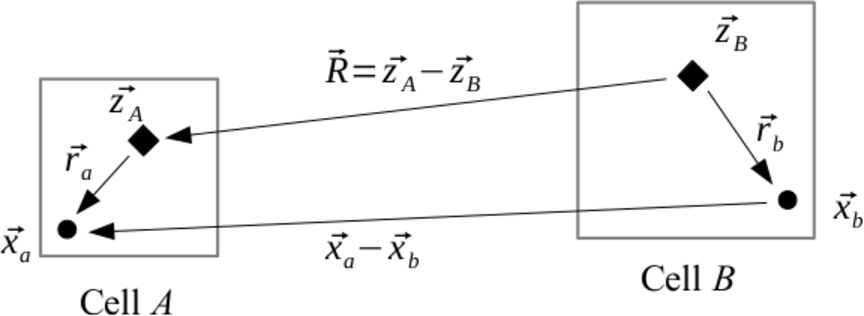
\includegraphics[width=\columnwidth]{cells.pdf}
\caption{The basics of the FMM: The potential generated by a particle
  at position $\mathbf{x}_b$ on a particle at position at location
  $\mathbf{x}_a$ is replaced by a Taylor expansion of the potential
  around the distance vector $\mathbf{R}$ linking the two centres of mass
  ($\mathbf{z}_A$ and $\mathbf{z}_B$) of cell $A$ and $B$. The
  expansion converges towards the exact expression provided
  $|\mathbf{R}|>|\mathbf{r}_a + \mathbf{r}_b|$.}
\label{fig:fmm:cells}
\end{figure}

In what follows, we use the compact multi-index notation of
\cite{Dehnen2014} (repeated in appendix \ref{sec:multi_index_notation}
for completeness) to simplify expressions and ease comparisons with
other published work. $\mathbf{k}$, $\mathbf{m}$ and $\mathbf{n}$ are
multi-indices and $\mathbf{r}$, $\mathbf{R}$, $\mathbf{x}$,
$\mathbf{y}$ and $\mathbf{z}$ are vectors, whilst $a$ and $b$ are
particle indices. Note also that we make no assumption on the specific
functional form of the potential $\varphi$.\\
For a single pair of particles $a$ and $b$ located in cell $A$ and $B$
with centres of mass $\mathbf{z}_A$ and $\mathbf{z}_B$ respectively,
as shown on Fig.~\ref{fig:fmm:cells}, the potential generated by $b$
at the location of $a$ can be rewritten as
\begin{align}
  \varphi(\mathbf{x}_a - \mathbf{x}_b)
  &= \varphi\left(\mathbf{x}_a - \mathbf{z}_A - \mathbf{x}_b +
  \mathbf{z}_B + \mathbf{z}_A - \mathbf{z}_B\right)  \nonumber \\
  &= \varphi\left(\mathbf{r}_a - \mathbf{r}_b + \mathbf{R}\right)
  \nonumber \\
  &= \sum_\mathbf{k} \frac{1}{\mathbf{k}!} \left(\mathbf{r}_a -
  \mathbf{r}_b\right)^{\mathbf{k}} \nabla^{\mathbf{k}}\varphi(\mathbf{R})
  \nonumber \\
  &= \sum_\mathbf{k} \frac{1}{\mathbf{k}!} \sum_{\mathbf{n} <
    \mathbf{k}} \binom{\mathbf{k}}{\mathbf{n}} \mathbf{r}_a^{\mathbf{n}}
  \left(-\mathbf{r}_b\right)^{\mathbf{k} - \mathbf{n}}
  \nabla^{\mathbf{k}}\varphi(\mathbf{R})\nonumber \\
  &= \sum_\mathbf{n} \frac{1}{\mathbf{n}!} \mathbf{r}_a^{\mathbf{n}}
  \sum_\mathbf{m} \frac{1}{\mathbf{m}!}
  \left(-\mathbf{r}_b\right)^\mathbf{m} \nabla^{\mathbf{n}+\mathbf{m}} \varphi(\mathbf{R}),
  \label{eq:fmm:expansion}
\end{align}
where we used the Taylor expansion of $\varphi$ around $\mathbf{R} \equiv
\mathbf{z}_A - \mathbf{z}_B$ on the third line, used $\mathbf{r}_a
\equiv \mathbf{x}_a - \mathbf{z}_A$, $\mathbf{r}_b \equiv \mathbf{x}_b
- \mathbf{z}_B$ throughout and defined $\mathbf{m} \equiv
\mathbf{k}-\mathbf{n}$ on the last line. Expanding the series only up
to order $p$, we get
\begin{equation}
  \varphi(\mathbf{x}_a - \mathbf{x}_b) \approx \sum_{\mathbf{n}}^{p}
  \frac{1}{\mathbf{n}!} \mathbf{r}_a^{\mathbf{n}} \sum_{\mathbf{m}}^{p
    -|\mathbf{n}|} 
  \frac{1}{\mathbf{m}!} \left(-\mathbf{r}_b\right)^\mathbf{m}
  \nabla^{\mathbf{n}+\mathbf{m}} \varphi(\mathbf{R}),
  \label{eq:fmm:fmm_one_part}
\end{equation}
with the approximation converging as $p\rightarrow\infty$ towards the
correct value provided $|\mathbf{R}|>|\mathbf{r}_a +
\mathbf{r}_b|$. If we now consider all the particles within $B$ and
combine their contributions to the potential at location
$\mathbf{x}_a$ in cell $A$, we get
\begin{align}
  \phi_{BA}(\mathbf{x}_a) &= \sum_{b\in B}G m_b\varphi(\mathbf{x}_a -
  \mathbf{x}_b)  \label{eq:fmm:fmm_one_cell}  \\
  &\approx G\sum_{\mathbf{n}}^{p}
  \frac{1}{\mathbf{n}!} \mathbf{r}_a^{\mathbf{n}} \sum_{\mathbf{m}}
    ^{p -|\mathbf{n}|}
  \frac{1}{\mathbf{m}!} \sum_{b\in B} m_b\left(-\mathbf{r}_b\right)^\mathbf{m}
  \nabla^{\mathbf{n}+\mathbf{m}} \varphi(\mathbf{R}) \nonumber. 
\end{align}
This last equation forms the basis of the FMM. The algorithm
decomposes the equation into three separated sums evaluated at
different stages.\\

\subsubsection{The FMM algorithm}

In a first step, multipoles are constructed from the
innermost sum. For each cell, we compute all the terms
\begin{equation}
  \mathsf{M}_{\mathbf{m}}(\mathbf{z}_B) = \frac{1}{\mathbf{m}!}
  \sum_{b\in B} m_b\left(-\mathbf{r}_b\right)^\mathbf{m} \label{eq:fmm:P2M} 
\end{equation}
up to order $p$. This is the first kernel of the method, commonly
labelled as \textsc{P2M} (particle to multipole). In a second step, we
compute the second kernel, \textsc{M2L} (multipole to local
expansion), which corresponds to the interaction of a cell with
another one:
\begin{equation}
  \mathsf{F}_{\mathbf{n}}(\mathbf{z}_A) = G\sum_{\mathbf{m}}^{p -|\mathbf{n}|}
  \mathsf{M}_{\mathbf{m}}(\mathbf{z}_B)
  \mathsf{D}_{\mathbf{n}+\mathbf{m}}(\mathbf{R}), \label{eq:fmm:M2L} 
\end{equation}
where $\mathsf{D}_{\mathbf{n}+\mathbf{m}}(\mathbf{R}) \equiv
\nabla^{\mathbf{n}+\mathbf{m}} \varphi(\mathbf{R})$ is an order $n+m$
derivative of the potential. This is the computationally expensive
step of the FMM algorithm as the number of operations in a naive
implementation using cartesian coordinates scales as
$\mathcal{O}(p^6)$. More advanced techniques
\citep[e.g.][]{Dehnen2014} can bring the cost down to
$\mathcal{O}(p^3)$, albeit at a considerable algebraic cost. For
collisionless dynamics, high accuracy is not required and low values
of $p$ are sufficient, which maintains the computational cost of the
M2L kernel at a reasonable level.  
Finally, in the last step, the potential is propagated from the local
expansion centre to the particles (L2P kernel) using
\begin{equation}
  \phi_{BA}(\mathbf{x}_a) = \sum_{\mathbf{n}}^{p}
  \frac{1}{\mathbf{n}!} \mathbf{r}_a^{\mathbf{n}}
  \mathsf{F}_{\mathbf{n}}(\mathbf{z}_A). \label{eq:fmm:L2P} 
\end{equation}
In summary, the potential generated by a cell $B$ on the particles in
cell $A$ is obtained by the successive application of the P2M, M2L and
L2P kernels. The P2M and L2P kernels are applied only once per
particle, whilst one M2L calculation has to be performed for each pair
of cells. The forces applied to the particles are obtained by the same
procedure using an extra order in the Taylor expansion. For instance,
for the acceleration along $x$, we have:
\begin{equation}
  a_x(\mathbf{x}_a) = \sum_{\mathbf{n}}^{p-1}
  \frac{1}{\mathbf{n}!} \mathbf{r}_a^{\mathbf{n}}
  \mathsf{F}_{\mathbf{n}+\left(1,0,0\right)}(\mathbf{z}_A). \label{eq:fmm:L2P_force} 
\end{equation}
In practice, the multipoles can be constructed recursively from the
leaves of the tree to the root and the local expansions from the root
to the leaves by shifting the $\mathsf{M}$ and $\mathsf{F}$ tensors
and adding their contributions to their parent or daughter cell's
tensors respecitvely. The shifting formulas (M2M and L2L kernels)
read:

\begin{align}
  \mathsf{M}_{\mathbf{m}}(\mathbf{x} + \mathbf{y}) &=
  \sum_{\mathbf{n}}^{\mathbf{m}}
  \frac{\mathbf{y}^\mathbf{n}}{\mathbf{n}!}\mathsf{M}_{\mathbf{m} -
    \mathbf{n}}(\mathbf{x}), \label{eq:fmm:M2M} \\
  \mathsf{F}_{\mathbf{n}}(\mathbf{x} + \mathbf{y}) &=
  \sum_{\mathbf{m}}^{p-|\mathbf{n}|}
  \frac{\mathbf{y}^\mathbf{m}}{\mathbf{m}!}\mathsf{F}_{\mathbf{m} +
    \mathbf{n}}(\mathbf{x}). \label{eq:fmm:L2L} 
\end{align}
One final, useful expression that enters some interaction between
tree-leaves is the P2M kernel that directly applies the potential due
to a multipole expansion to a particle without using the expansion of
the potential $\mathsf{F}$ at the centre of mass of the cell. This
kernel is obtained by setting $\mathbf{r}_a$ to zero in
eq.~\ref{eq:fmm:expansion}, re-defining
$\mathbf{R}\equiv\mathbf{x}_{\rm a} - \mathbf{z}_{\rm B}$ and
constructing the same $\mathsf{M}$ and $\mathsf{D}$ tensor than for
the other kernels:
\begin{align}
  \phi_{Ba}(\mathbf{x}_a) &= G\sum_{\mathbf{m}}^p \mathsf{M}_{\mathbf{m}} \mathsf{D}_{\mathbf{m}}(\mathbf{R}),\\
  a_x(\mathbf{x}_a) &= G\sum_{\mathbf{m}}^p \mathsf{M}_{\mathbf{m}} \mathsf{D}_{\mathbf{m}+\left(1,0,0\right)}(\mathbf{R}).
  \label{eq:fmm:M2P}
\end{align}
A traditional tree-code uses solely that kernel to obtain the forces
from the multipoles (or often just monopoles, i.e. setting $p=0$ throughout)
to the particles.\\
All the kernels (Eqs.~\ref{eq:fmm:P2M}-\ref{eq:fmm:M2P}) are rather
straightforward to evaluate as they are only made of additions and
multiplications (provided $\mathsf{D}$ can be evaluated quickly),
which are extremely efficient instructions on modern architectures
(see Appendix \ref{sec:pot_derivatives} for the full
expressions). However, the fully expanded sums can lead to rather
large and prone to typo expressions. To avoid any mishaps, we use a
\texttt{python} script to generate C code in which all the sums are
unrolled and correct by construction. In \swift, we implemented the
kernels up to order $p=5$, as it proved to be accurate enough for our
purpose, but this could be extended to higher order easily. This
implies storing $56$ numbers per cell for each $\textsf{M}$ and
$\textsf{F}$ plus three numbers for the location of the centre of
mass. For leaf-cells with large numbers of particles, as in \swift,
this is a small memory overhead. One further small improvement
consists in choosing $\mathbf{z}_A$ to be the centre of mass of cell
$A$ rather than its geometrical centre. The first order multipoles
($\mathsf{M}_{100},\mathsf{M}_{010},\mathsf{M}_{001}$) then vanish by
construction. This allows us to simplify some of the expressions and
helps reduce, albeit by a small fraction, the memory footprint of the
tree structure.

\subsubsection{The Multipole acceptance criterion}

%\subsection{Notes on the derivatives of the gravitational potential}
\label{ssec:grav_derivatives}

The calculation of all the
$\mathsf{D}_\mathbf{n}(x,y,z) \equiv \nabla^{\mathbf{n}}\phi(x,y,z)$ terms up
to the relevent order can be quite tedious and it is beneficial to
automatize the whole setup. Ideally, one would like to have an
expression for each of these terms that is only made of multiplications
and additions of each of the coordinates and the inverse distance. We
achieve this by writing $\phi$ as a composition of functions
$\phi(u(x,y,z))$ and apply the \textit{Fa\`a di Bruno}
formula \citep[i.e. the ``chain rule'' for higher order derivatives,
 see e.g.][]{Hardy2006} to construct our terms:
\begin{equation}
\label{eq:faa_di_bruno}
\frac{\partial^n}{\partial x_1 \cdots \partial x_n} \phi(u)
= \sum_{A} \phi^{(|A|)}(u) \prod_{B \in
A} \frac{\partial^{|B|}}{\prod_{c\in B}\partial x_c} u(x,y,z),
\end{equation}
where $A$ is the set of all partitions of $\lbrace1,\cdots, n\rbrace$,
$B$ is a block of a partition in the set $A$ and $|\cdot|$ denotes the
cardinality of a set. For generic functions $\phi$ and $u$ this
formula yields an untracktable number of terms; an 8th-order
derivative will have $4140$ (!)  terms in the sum\footnote{The number
  of terms in the sum is given by the Bell number of the same
  order.}. \\ For the un-softened gravitational potential, we choose to write
\begin{align}
   \phi(x,y,z) &= 1 / \sqrt{u(x,y,z)}, \\
   u(x,y,z) &= x^2 + y^2 + z^2.
\end{align}
This choice allows to have derivatives of any order of $\phi(u)$ that
can be easily expressed and only depend on powers of $u$:
\begin{equation}
\phi^{(n)}(u) = (-1)^n\cdot\frac{(2n-1)!!}{2^n}\cdot\frac{1}{u^{n+\frac{1}{2}}},
\end{equation}
where $!!$ denotes the semi-factorial. More importantly, this
choice of decomposition allows us to have non-zero derivatives of $u$
only up to second order in $x$, $y$ or $z$. The number of non-zero
terms in eq. \ref{eq:faa_di_bruno} is hence drastically reduced. For
instance, when computing $\mathsf{D}_{(4,1,3)}(\mathbf{r}) \equiv
\frac{\partial^8}{\partial x^4 \partial y \partial z^3}
\phi(u(x,y,z))$, $4100$ of the $4140$ terms will involve at least one
zero-valued derivative (e.g. $\partial^3/\partial x^3$ or
$\partial^2/\partial x\partial y$) of $u$. Furthermore, among the 40
remaining terms, many will involve the same combination of derivatives
of $u$ and can be grouped together, leaving us with a sum of six
products of $x$,$y$ and $z$. This is generally the case for most of
the $\mathsf{D}_\mathbf{n}$'s and figuring out which terms are identical in a
given set of partitions of $\lbrace1,\cdots, n\rbrace$ is an
interesting exercise in combinatorics left for the reader \citep[see
  also][]{Hardy2006}. We use a \texttt{python} script based on this
technique to generate the actual C routines used within \swift. Some
examples of these terms are given in Appendix
\ref{sec:pot_derivatives}.


\subsection{Coupling the FMM to a mesh for periodic long-range forces}
\label{ssec:mesh_summary}

\begin{equation}
  S(x) = \frac{e^x}{1 + e^x}
\end{equation}

\begin{align}
  \varphi_s(r) &= \frac{1}{r}\left[2 - 2S\left(\frac{2r}{r_s}\right)\right] \nonumber\\
  &= \frac{1}{r}\left[2 - \frac{2e^{\frac{2r}{r_s}}}{1+e^{\frac{2r}{r_s}}}\right] 
\end{align}
\begin{align}
  |\mathbf{f}_s(r)| &= \frac{1}{r^2}\left[\frac{4r}{r_s}S'\left(\frac{2r}{r_s}\right) - 2S\left(\frac{2r}{r_s}\right) + 2\right] \nonumber \\
  &= \frac{1}{r^2}\left[\frac{4r}{r_s}\frac{e^{\frac{2r}{r_s}}}{(1+e^{\frac{2r}{r_s}})^2} - \frac{2e^{\frac{2r}{r_s}}}{1+e^{\frac{2r}{r_s}}} + 2\right]
\end{align}

\begin{equation}
  \tilde\varphi_l(k) = \frac{1}{k^2}\left[\frac{\upi}{2}kr_s\textrm{csch}\left(\frac{\upi}{2}kr_s\right) \right]
\end{equation}

\begin{figure}
\includegraphics[width=\columnwidth]{potential_short.pdf}
\caption{aa}
\label{fig:fmm:potential_short}
\end{figure}


\begin{figure}
\includegraphics[width=\columnwidth]{force_short.pdf}
\caption{bb}
\label{fig:fmm:force_short}
\end{figure}


\begin{figure}
\includegraphics[width=\columnwidth]{potential_long.pdf}
\caption{cc}
\label{fig:fmm:potential_long}
\end{figure}

\subsection{The multipole acceptance criterion}

The main remaining question is to decide when two cells are far enough from
each others that the truncated Taylor expansion used as approximation for
the potential (eq. \ref{eq:fmm:expansion}) is accurate enough. The
criterion used to make that decision is called the \emph{multipole
  acceptance criterion} (MAC). \\
We know that (\ref{eq:fmm:expansion}) is converging towards the correct
answer provided $1>|\mathbf{r}_a + \mathbf{r}_b| / |\mathbf{R}|$. This is
hence the most basic (and always necessary) MAC that can be designed. If
this ratio is lower, the accuracy (at a fixed expansion order) is improved
and it is hence common practice to define a critical \emph{opening angle}
$\theta_{\rm cr}$ and allow the use of the multipole approximation between
two cells if

\begin{equation}
  \theta_{\rm cr} > \frac{\rho_A + \rho_B} {|\mathbf{R}|}.
  \label{eq:fmm:angle}
\end{equation}
This lets users have a second handle on the accuracy on the gravity
calculation besides the much more involved change in the expansion order
$p$ of the FMM method. Typical values for the opening angle are in the
range $[0.3, 0.7]$, with the cost of the simulation growing as $\theta_{\rm
  cr}$ decreases. \\
This method has the drawback of using a uniform criterion across the entire
simulation volume and time evolution, which means that the chosen value of
$\theta_{\rm cr}$ could be too small in some regions (leading to too many
operations for the expected accuracy) and too large in some other other
ones (leading to a lower level of accuracy than expected). \swift instead
uses a more adaptive criterion to decide when the multipole approximation
can be used. This is based on the error analysis of FMM by
\cite{Dehnen2014} and is summarised below for completeness. The key idea is
to exploit the additional information about the distribution of particles
that is encoded in the higher-order multipole terms.\\
We start by defining the scalar quantity $P_{A,n}$, the
\emph{power} of the multipole of order $n$ of the particles in cell $A$,
via
\begin{equation}
  P_{A,n}^2 = \sum_{|\mathbf{m}|=n} \frac{\mathbf{m}!}{|\mathbf{m}|!}\mathsf{M}_{A,\mathbf{m}}^2,
\end{equation}
where the sum runs over all the multipole terms of order $n$ in the
cell\footnote{Note that $P_{0} \equiv \mathsf{M}_{(0,0,0)}$ is
  just the mass of the cell and since \swift uses the centre of mass as the
  centre of expansion of the multipoles, $P_{1} = 0$.}. This
quantity is a simple upper bound for the amplitude of the multipole
($\mathsf{M}_{A, \mathbf{m}} < P_{A,|\mathbf{m}|}/|\mathbf{m}|!$)
and can hence be used to estimate the importance of the terms of a given
order in the Taylor series of the potential. Following \cite{Dehnen2014} we
then consider a sink cell $A$ and a source cell $B$ (figure \ref{fig:fmm:cells}) for which we evaluate
at order $p$ the scalar
\begin{equation}
  E_{BA,p} = \frac{1}{M_B|\mathbf{R}|^p} \sum_{n=0}^p \binom{p}{n} P_{B,n}
  \rho_A^{p-n},
  \label{eq:fmm:e_ab}
\end{equation}
with $M_B \equiv \mathsf{M}_{B,(0,0,0)}$, the sum of the mass of the
particles in cell $B$. Note that since $P_{B,n} \leq M_B
\rho_B^n$, we have $E_{BA, p} \leq \left((\rho_A +
\rho_B)/|\mathbf{R}|\right)^p$, where the right-hand side is the
expression used in the basic opening angle condition
(\ref{eq:fmm:angle}). We finally scale the $E_{BA,p}$'s by the relative
size of the two cells to define the error estimator $\tilde{E}_{BA,p}$:
\begin{equation}
  \tilde{E}_{BA,p} = 8\frac{\max(\rho_A, \rho_B)}{\rho_A + \rho_B}E_{BA,p}.
  \label{eq:fmm:e_ab_tilde}
\end{equation}
As shown by \cite{Dehnen2014}, these quantities are excellent estimators of
the error made in computing the accelerations between two cells using the
M2L and M2P kernels at a given order. We can hence use this property to
design a new MAC by demanding that the estimated acceleration error is no
larger than a certain fraction of the smallest acceleration in the sink
cell $A$. This means we can use the FMM approximation between to
approximate the accelerations in cell $A$ due to the particles in cell $B$ if
\begin{equation}
  \tilde{E}_{BA,p} \frac{M_B}{|\mathbf{R}|^2} < \epsilon_{\rm FMM} \min_{a\in
    A}\left(|\mathbf{a}_a|\right) \quad \rm{and} \quad \frac{\rho_A +
    \rho_B} {|\mathbf{R}|} < 1,
  \label{eq:fmm:mac}  
\end{equation}
where the $\mathbf{a}_a$ are the accelerations of the particles in cell $A$
and $\epsilon_{\rm FMM}$ is a tolerance parameter. Since this is self-referencing
(i.e. we need the accelerations to decide how to compute the
accelerations), we need to use a an estimator of $|\mathbf{a}_a|$. In
\swift, we follow the strategy used by \gadget and use the acceleration of
the previous time-step\footnote{On the first time-step of a simulation this
  value has not been computed yet. We hence run a fake 0th time-step with
  the simpler MAC (eq. \ref{eq:fmm:angle}), which is good enough to obtain
  approximations of the accelerations.}. The minimal norm of the
acceleration in a given cell can be computed at the same time as the P2M
and M2M kernels are evaluated in the tree construction phase. The second
condition in (\ref{eq:fmm:mac}) is necessary to ensure the convergence of the
Taylor expansion.\\
One important difference between this criterion and the purely
geometric one (\ref{eq:fmm:angle}) is that it is not symmetric in $A
\leftrightarrow B$ (i.e. $E_{AB,p} \neq E_{BA,p}$). This implies that
there are cases where a multipole in cell $A$ can be used to compute
the field tensors in cell $B$ but the multipole in $B$ cannot be used
to compute the $\mathsf{F}$ values of cell $A$ and vice versa. This
affects the tree walk by breaking the symmetry and potentially leading
to cells of different sizes interacting. \\
For the M2P kernel, the sink is a single particle $a$ and hence
$\rho_A = 0$, which simplifies some of the expressions above. In this
case, at order $p$, we get:
\begin{equation}
  E_{BA,p} = \frac{P_{B,p}}{M_B |\mathbf{R}|^p}, \qquad
  \tilde{E}_{BA,p} = 8E_{BA,p} \nonumber
\end{equation}
Note that, in this case, only the power term of the order of the
scheme appears; not a sum over the lower-order ones. This leads to the
following MAC for the M2P kernel:
\begin{equation}
  8\frac{P_{B,p}}{|\mathbf{R}|^{p+2}} < \epsilon_{\rm FMM} |\mathbf{a}_a| \quad
  \rm{and} \quad \frac{\rho_B} {|\mathbf{R}|} < 1.
    \label{eq:fmm:mac_m2p}  
\end{equation}
The value of $\epsilon_{\rm FMM}$ could in principle be different than the one
used for the M2L MAC. One special case is of particular interest to
link our expression to other results. Using the expression for order
$2$ and the approximation $P_{B,p} \approx M_B \rho_B^p$, we
get
\begin{equation}
  8\frac{M_B}{|\mathbf{R}|^2}\left(\frac{\rho_B}{|\mathbf{R}|}\right)^2
  < \epsilon_{\rm FMM} |\mathbf{a}_a| \nonumber
\end{equation}
for our MAC.  This is the same expression as the adaptive opening
angle used by \gadget \cite[see eq.18 of][]{Springel2005} up to
numerical factors and definition of the size of a multipole ($\rho$
vs. the cell edge). Note, however, that, in practice, since formally
$P_{B,p} \leq M_B \rho_B^p$, the dependence is slightly
different.\\
We conclude this section by noting that whilst the derivation of the
FMM equations and of the simple geometric MAC (eq. \ref{eq:fmm:angle})
do not make any assumptions about the functional form of $\varphi(r)$,
the more advanced MAC is valid in the specific case of the
gravitational potential $\varphi(r) = m/r$ as can be inferred from the
$m/r^2$ term appearing on the LHS of the criteria (\ref{eq:fmm:mac})
and (\ref{eq:fmm:mac_m2p}).

\subsubsection{Modifications for softened and truncated gravity}

\begin{figure}
\includegraphics[width=\columnwidth]{mac_potential.pdf}
\caption{The gravitational forces $f_{\rm SWIFT}$ computed by SWIFT
  (green line) including the force softening on the smallest scales
  and the long-range periodic mesh truncation on the largest scales
  for a simulation box of size $L$, a mesh scale-length $r_s$ and
  Plummer-equivalent softening $\epsilon_{\rm Plummer}$. The
  approximate fast estimator of the forces used in the MAC $f_{\rm
    MAC}$ is shown using yellow dash-dotted lines. Note that, by
  construction, $f_{\rm SWIFT} \leq f_{\rm MAC} \leq 1/r^2$ for all
  distances $r$.}
\label{fig:fmm:mac_potential}
\end{figure}

One drawback of using expression (\ref{eq:fmm:mac}) in the case of a
softened potential (or a potential truncated to apply long-range
forces from a mesh (Sec. \ref{ssec:mesh_summary}) is that the $M/R^2$
term will overestimate the expected contribution from the multipole to
the filed tensors, sometimes by large factors. This difference is
shown on fig. \ref{fig:fmm:mac_potential}, with for instance a ratio
of $3$ between the true forces and the Newtonian values reached a the
scale of the Plummer softening. Using the simple expression
(\ref{eq:fmm:mac}) will make the MAC too aggressive by preventing it
from using a given multipole as it will be difficult to make the large
term $M/R^2$ be below the fixed fraction $\epsilon_{\rm FMM}$ of the
total acceleration of the receiving cell. This implies more
computation as it will force the tree-walk algorithm to use more
interactions by going to the daughter cells. The estimation of the
contribution of the multipole in the MAC should hence be replaced by a
more realistic term, closer to the one actually used in the
interactions (eq. \ref{eq:fmm:force_norm}). In simulations with
periodic boundary conditions, the same reasoning applies to the
truncated force at the radii overlapping with the scale $r_s$ of the
mesh forces.

However, both the short- and long-range truncation functions are
expensive to evaluate in the context of the MAC which is called a
large number of times during a tree walk. We hence, construct a
cheaper to evaluate estimator $f_{\rm MAC}$ that is closer to the true
forces than the purely Newtonian term:
\begin{align}
f_{\rm MAC}(r) =
\left\lbrace\begin{array}{rcl}
  \left(\frac{9}{5}\right)^2 H^{-2} & \mbox{if} & r <
  \frac{5}{9}H,\\
  r^{-2} & \mbox{if} & \frac{5}{9}H \leq r < \frac{5}{3}r_s, \\
  \left(\frac{5}{3}\right)^2 r_s^2 r^{-4} & \mbox{if} & \frac{5}{3}r_s \leq r. \\
\end{array}
\right.
\label{eq:fmm:f_mac}
\end{align}
Since it is made of constants and even powers of the distance,
computin this term is much cheaper than the true forces.  This
esimator is shown as a dot-dashed line on
Fig. \ref{fig:fmm:mac_potential} and obeys the relation $f_{\rm
  SWIFT}(r) \leq f_{\rm MAC}(r) \leq 1/r^2$, with $f_{\rm SWIFT}(r)$
being the true truncated and softened norm of the gravity forces the
code solves for (green line). We use this expression in the multipole
acceptance criterion instead of the $1/|\mathbf{R}|$ term:
\begin{equation}
  \tilde{E}_{BA,p} M_Bf_{\rm MAC}(|\mathbf{R}|) < \epsilon_{\rm FMM} \min_{a\in
    A}\left(|\mathbf{a}_a|\right).
  \label{eq:fmm:mac_f_mac}  
\end{equation}
The same change is applied to the MAC used for the M2P kernel
(eq. \ref{eq:fmm:mac_m2p}). In the non-truncated un-softened case,
their expressions reduce to the \citep{Dehnen2014} one. Using this
$f_{\rm MAC}$ instead of the simpler purely-Newtonian one only makes a
difference in simulations where a lot of particles cluster below the
scale of the softening, which is often the case for hydrodynamical
simulations including radiative cooling processes. The use of this
term over the simpler $1/r^2$ estimator is a runtime parameter.


\subsection{Exact forces for accuracy checks}
\label{ssec:exact_forces}

To assess the accuracy of the gravity solver, \swift can also compute
the gravitational forces and potential for a subset of particles using
a simple direct summation method. This is obviously much slower and
should only be used for code testing purposes. The forces for a
selection of particles are computed every time-step if they are active
and dumped to a file alongside the forces computed by the FMM method.

In the case where periodic boundary conditions are used, we apply the
\cite{Ewald1921} summation technique to include the contribution to
the forces of all the infinite periodic replications of the particle
distribution. We use the approximation to the infinite series of terms
proposed by \cite{Hernquist1991}\footnote{Note, however, that there is
a typo in their formula for the force correction terms. The correct
expression is given by \cite{Klessen1997} \citep[see
also][]{Hubber2011}.}, which we tabulate in one octant using 64
equally spaced bins along each spatial direction spanning and the
range $[0,L]$, where $L$ is the side-length of the box.


\bibliographystyle{mnras}
\bibliography{./bibliography.bib}

\appendix
\section{Multi-index notation}
\label{sec:multi_index_notation}

We define a multi-index $\mathbf{n}$ as a triplet of integers
non-negative integers:
\begin{equation}
  \mathbf{n} \equiv \left(n_x, n_y, n_z\right), \qquad n_i \in \mathbb{N},
\end{equation}
with a norm $n$ given by
\begin{equation}
  n = |\mathbf{n}| \equiv n_x + n_y + n_z. 
\end{equation}
We also define the exponentiation of a vector
$\mathbf{r}=(r_x,r_y,r_z)$ by a multi-index $\mathbf{n}$ as
\begin{equation}
  \mathbf{r}^\mathbf{n} \equiv r_x^{n_x} \cdot r_y^{n_y} \cdot r_z^{n_z},
\end{equation}
which for a scalar $\alpha$ reduces to
\begin{equation}
  \alpha^\mathbf{n} = \alpha^{n}.
\end{equation}
Finally, the factiorial of a multi-index is defined to be
\begin{equation}
  \mathbf{n}! \equiv n_x! \cdot n_y! \cdot n_z!,
\end{equation}
which leads to a simple expression for the binomial coefficients of
two multi-indices entering Taylor expansions:
\begin{equation}
  \binom{\mathbf{n}}{\mathbf{k}} = \binom{n_x}{k_x}\binom{n_y}{k_y}\binom{n_z}{k_z}.
\end{equation}
When appearing as the index in a sum, a multi-index represents all
values that the triplet can take up to a given norm. For instance,
$\sum_{\mathbf{n}}^{p}$ indicates that the sum runs over all possible
multi-indices whose norm is $\leq p$.

\onecolumn
\section{Derivatives of the potential}
\label{sec:pot_derivatives}

For completeness, we give here the full expression for the first few
derivatives of the potential that are used in our FMM scheme. We use
the notation $\mathbf{r}=(r_x, r_y, r_z)$, $r = |\mathbf{r}|$, $u=r/H$
and $x=2r/r_s$. We also assume $H \ll r_s$. We can construct the
higher order derivatives by successively applying the "chain rule". We
show representative examples of the first few relevant ones here split
by order. We start by constructing derivatives of the truncated
potentials. The first step is the construction of derivatives of the
long-range truncation function. We define
\begin{equation}
  \alpha(w) \equiv \left(1 + e^w\right)^{-1} \nonumber
\end{equation}
and compute its derivatives in terms of powers of $\alpha$ (note the
difference in notation between powers $\alpha^n$ and n-th derivatives
$\alpha^{(n)}$)\footnote{This can be computed by \textsc{Mathematica}
  using the expression \texttt{Apart[D[1/(1 + Exp[w]), {w, n}]]} for
  the n-th derivative.}:
\begin{align}
  \alpha^{(0)}(w) &= +\alpha(w), \nonumber\\
  \alpha^{(1)}(w) &= -\alpha(w) + \alpha^2(w),  \nonumber\\
  \alpha^{(2)}(w) &= +\alpha(w) - 3\alpha^2(w) + 2\alpha^3(w),  \nonumber\\
  \alpha^{(3)}(w) &= -\alpha(w) + 7\alpha^2(w) - 12\alpha^3(w) + 6\alpha^4(w),   \nonumber\\
  \alpha^{(4)}(w) &= +\alpha(w) - 15\alpha^2(w) + 50\alpha^3(w) - 60\alpha^4(w) + 24\alpha^5(w),    \nonumber\\
  \alpha^{(5)}(w) &= -\alpha(w) + 31\alpha^2(w) -180\alpha^3(w) + 390\alpha^4(w) -360\alpha^5(w) + 120\alpha^6(w).\nonumber                                      
\end{align}
We can then construct our sigmoid $\sigma(w) \equiv e^w\alpha(w)$ and
its derivatives, again in terms of powers of $\alpha(w)$ only:
\begin{align}
  \sigma^{(0)}(w) &= e^w\alpha(w), \nonumber\\
  \sigma^{(1)}(w) &= e^w\left(\alpha^{(1)}(w) + \alpha(w) \right) \nonumber\\
                  &= e^w \alpha^2(w), \nonumber \\
  \sigma^{(2)}(w) &= e^w\left(\alpha(w) +2\alpha^{(1)}(w) + \alpha^{(2)}(w)  \right) \nonumber\\
                  &= e^w \left(2\alpha^3(w) - \alpha^2(w)\right), \nonumber \\
  \sigma^{(3)}(w) &= e^w\left(\alpha(w) + 3\alpha^{(1)}(w) + 3\alpha^{(2)}(w) + \alpha^{(3)}(w)  \right) \nonumber\\
                  &= e^w \left(6\alpha^4(w) - 6\alpha^3(w) + \alpha^2(w)\right), \nonumber \\
  \sigma^{(4)}(w) &= e^w\left(\alpha(w) + 4\alpha^{(1)}(w) + 6\alpha^{(2)}(w) + 4\alpha^{(3)}(w) + \alpha^{(4)}(w)  \right) \nonumber\\
                  &= e^w \left(24\alpha^5(w) - 36\alpha^4(w) + 14\alpha^3(w) - \alpha^2(w)\right), \nonumber \\
  \sigma^{(5)}(w) &= e^w\left(\alpha(w) + 5\alpha^{(1)}(w) + 10\alpha^{(2)}(w) + 10\alpha^{(3)}(w) + 5\alpha^{(4)}(w) + \alpha^{(5)}(w)  \right) \nonumber\\
                  &= e^w \left(120\alpha^6(w) - 240\alpha^5(w) + 150\alpha^4(w) - 30\alpha^3(w) + \alpha^2(w)\right). \nonumber 
\end{align}
We can finally construct our long-range truncation function
$\chi(r,r_s) \equiv 2 - 2\sigma(2r/r_s)$ and its derivatives
\begin{align}
  \chi(r,r_s) &= 2 - 2e^{2r/r_s} \alpha(2r/r_s), \nonumber \\
  \frac{\partial}{\partial r} \chi(r, r_s) &= -2 \left(\frac{2}{r_s}\right)^1 \sigma^{(1)}\left(\frac{2r}{r_s}\right) = -2 \left(\frac{2}{r_s}\right)^1 e^{\frac{2r}{r_s}} \alpha^2 \left(\frac{2r}{r_s}\right), \nonumber\\
  \frac{\partial^2}{\partial r^2} \chi(r, r_s) &= -2 \left(\frac{2}{r_s}\right)^2 \sigma^{(2)}\left(\frac{2r}{r_s}\right) = -2 \left(\frac{2}{r_s}\right)^2  e^{\frac{2r}{r_s}} \left[2\alpha^3 \left(\frac{2r}{r_s}\right) - \alpha^2 \left(\frac{2r}{r_s}\right) \right], \nonumber\\
  \frac{\partial^3}{\partial r^3} \chi(r, r_s) &= -2 \left(\frac{2}{r_s}\right)^3 \sigma^{(3)}\left(\frac{2r}{r_s}\right) = -2 \left(\frac{2}{r_s}\right)^3  e^{\frac{2r}{r_s}} \left[6\alpha^4 \left(\frac{2r}{r_s}\right) - 6\alpha^3 \left(\frac{2r}{r_s}\right) + \alpha^2 \left(\frac{2r}{r_s}\right) \right],\nonumber \\
  \frac{\partial^4}{\partial r^4} \chi(r, r_s) &= -2 \left(\frac{2}{r_s}\right)^4 \sigma^{(4)}\left(\frac{2r}{r_s}\right) = -2 \left(\frac{2}{r_s}\right)^4  e^{\frac{2r}{r_s}} \left[24\alpha^5 \left(\frac{2r}{r_s}\right) - 36\alpha^4 \left(\frac{2r}{r_s}\right) + 14\alpha^3 \left(\frac{2r}{r_s}\right) - \alpha^2 \left(\frac{2r}{r_s}\right) \right],\nonumber \\
  \frac{\partial^5}{\partial r^5} \chi(r, r_s) &= -2 \left(\frac{2}{r_s}\right)^5 \sigma^{(5)}\left(\frac{2r}{r_s}\right) = -2 \left(\frac{2}{r_s}\right)^5  e^{\frac{2r}{r_s}} \left[120\alpha^6 \left(\frac{2r}{r_s}\right) - 240\alpha^5 \left(\frac{2r}{r_s}\right) + 150\alpha^4 \left(\frac{2r}{r_s}\right) - 30\alpha^3 \left(\frac{2r}{r_s}\right) + \alpha^2 \left(\frac{2r}{r_s}\right) \right].\nonumber
\end{align}
In the Newtonian limit ($r_s\rightarrow\infty$) the first expression
reduces to $\chi(r,r_s) = 1$ whilst all higher-order derivatives
vanish. In the limit $r\rightarrow\infty$ (and $r_s < \infty$), all terms vanish. All these
derivatives can be computed easily as they are simple polynomials of
$\alpha(2r/r_s)$. They involve one exponential and one inversion for
the initial calculation of $\alpha$ and all the other terms can be
obtained very eeficiently on modern architectures as they only involve
\emph{fused-multiple-add} operations.We can now construct common
quantities that appear in derivatives of multiple orders of the
truncated an softened gravity field $\varphi (\mathbf{r}, r_s, H)
\equiv \frac{1}{r}\chi(r,r_s)$:


% \begin{align}
%   \alpha(x) &= \left(1 + e^x\right)^{-1}  \nonumber \\
%   \chi(r, r_s) &= 2\left(1 - e^{2r/r_s}\alpha(2r/r_s) \right) \nonumber \\
%   \chi'(r, r_s) &= \frac{2}{r_s}\left(2\alpha(x)^2 - 2\alpha(x)\right) \nonumber \\
%   \chi''(r, r_s) &= \frac{4}{r_s^2}\left(4\alpha(x)^3 - 6\alpha(x)^2 + 2\alpha(x)\right) \nonumber \\
%   \chi^{(3)}(r, r_s) &= \frac{8}{r_s^3} \left(12\alpha(x)^4 - 24\alpha(x)^3 + 14\alpha(x)^2 -2 \alpha(x)\right) \nonumber \\
%   \chi^{(4)}(r, r_s) &= \frac{16}{r_s^4} \left(48\alpha(x)^5 - 120\alpha(x)^4 + 100\alpha(x)^3 -30 \alpha(x)^2 + 2\alpha(x)\right) \nonumber \\ 
%   \chi^{(5)}(r, r_s) &= \frac{32}{r_s^5} \left(240\alpha(x)^6 - 720\alpha(x)^5 + 780\alpha(x)^4 - 360\alpha(x)^3 + 62\alpha(x)^2 - 2\alpha(x) \right) \nonumber
% \end{align}

%%%%%%%%%%%%%%%%%%%%%%%%%%%%%%%%%%
\begin{align}
  \mathsf{\tilde{D}}_{1}(r, r_s, H) =
  \left\lbrace\begin{array}{rcl}
  \left(-3u^7 + 15u^6 - 28u^5 + 21u^4 - 7u^2 + 3\right)\times  H^{-1} & \mbox{if} & u < 1,\\
  %r^{-1} & \mbox{if} & u \geq 1,
  \chi(r, r_s) \times r^{-1} & \mbox{if} & u \geq 1,
  \end{array}
  \right.\nonumber
\end{align}
%%%%%%%%%%%%%%%%%%%%%%%%%%%%%%%%%%
\begin{align}
  \mathsf{\tilde{D}}_{3}(r, r_s, H) =
  \left\lbrace\begin{array}{rcl}
  -\left(21u^5 - 90u^4 + 140u^3 -84u^2 +14\right)\times  H^{-3}& \mbox{if} & u < 1,\\
  %-1 \times r^{-3} & \mbox{if} & u \geq 1,
  \left(r\chi'(r, r_s) - \chi(r, r_s)\right) \times r^{-3} & \mbox{if} & u \geq 1, 
  \end{array}
  \right.\nonumber
\end{align}
%%%%%%%%%%%%%%%%%%%%%%%%%%%%%%%%%%
\begin{align}
  \mathsf{\tilde{D}}_{5}(r, r_s, H) =
  \left\lbrace\begin{array}{rcl}
  \left(-105u^3 + 360u^2 - 420u + 168\right)\times  H^{-5}& \mbox{if} & u < 1,\\
  %3\times r^{-5} & \mbox{if} & u \geq 1,
  \left(r^2\chi''(r, r_s) - 3r\chi'(r, r_s) + 3\chi(r, r_s) \right)\times r^{-5} & \mbox{if} & u \geq 1, 
  \end{array}
  \right.\nonumber
\end{align}
%%%%%%%%%%%%%%%%%%%%%%%%%%%%%%%%%%
\begin{align}
  \mathsf{\tilde{D}}_{7}(r, r_s, H) =
  \left\lbrace\begin{array}{rcl}
  -\left(315u - 720 + 420u^{-1}\right)\times  H^{-7} & \mbox{if} & u < 1,\\
  %-15\times r^{-7} & \mbox{if} & u \geq 1,
  \left(r^3\chi^{(3)}(r, r_s) - 6r^2\chi''(r, r_s)+15r\chi'(r, r_s)-15\chi(r, r_s)\right) \times r^{-7} & \mbox{if} & u \geq 1, 
  \end{array}
  \right.\nonumber
\end{align}
%%%%%%%%%%%%%%%%%%%%%%%%%%%%%%%%%%
\begin{align}
  \mathsf{\tilde{D}}_{9}(r, r_s, H) =
  \left\lbrace\begin{array}{rcl}
  \left(-315u^{-1} + 420u^{-3}\right)\times  H^{-9}& \mbox{if} & u < 1,\\
  %105\times r^{-9} & \mbox{if} & u \geq 1.
  \left(r^4\chi^{(4)}(r, r_s) - 10r^3\chi^{(3)} + 45r^2\chi''(r, r_s) - 105r\chi'(r, r_s) + 105\chi(r, r_s) \right) \times r^{-9} & \mbox{if} & u \geq 1
  \end{array}
  \right.\nonumber
\end{align}
%%%%%%%%%%%%%%%%%%%%%%%%%%%%%%%%%%
\begin{align}
  \mathsf{\tilde{D}}_{11}(r, r_s, H) =
  \left\lbrace\begin{array}{rcl}
  -\left(315u^{-3} - 1260u^{-5}\right)\times  H^{-11}& \mbox{if} & u < 1,\\
  %-945\times r^{-11} & \mbox{if} & u \geq 1.
  \left(r^5\chi^{(5)}(r, r_s) - 15r^4\chi^{(4)}(r, r_s) + 105r^3\chi^{(3)}(r, r_s) - 420r^2\chi''(r, r_s) + 945r \chi'(r, r_s) - 945\chi(r, r_s)\right) \times r^{-11} & \mbox{if} & u \geq 1.
  \end{array}
  \right.\nonumber
\end{align}
%%%%%%%%%%%%%%%%%%%%%%%%%%%%%%%%%%
Starting from the potential (Eq. \ref{eq:fmm:potential},
reproduced here for completeness), we can now build all the relevent derivatives
\begin{align}
  \mathsf{D}_{000}(\mathbf{r}) = \varphi (\mathbf{r}, r_s, H) =
    \mathsf{\tilde{D}}_{1}(r, r_s, H) \nonumber
\end{align}

%%%%%%%%%%%%%%%%%%%%%%%%%%%%%%%%%%
\noindent\rule{6cm}{0.4pt}
\begin{align}
  \mathsf{D}_{100}(\mathbf{r}) = \frac{\partial}{\partial r_x} \varphi (\mathbf{r}, r_s, H) =
    r_x \mathsf{\tilde{D}}_{3}(r, r_s, H) \nonumber
\end{align}

%%%%%%%%%%%%%%%%%%%%%%%%%%%%%%%%%%
\noindent\rule{6cm}{0.4pt}
\begin{align}
\mathsf{D}_{200}(\mathbf{r}) = \frac{\partial^2}{\partial r_x^2} \varphi (\mathbf{r}, r_s, H) = 
r_x^2 \mathsf{\tilde{D}}_{5}(r, r_s, H) +
\mathsf{\tilde{D}}_{3}(r, r_s, H)\nonumber
\end{align}

\begin{align}
\mathsf{D}_{110}(\mathbf{r}) = \frac{\partial^2}{\partial r_x\partial r_y} \varphi (\mathbf{r}, r_s, H) = 
   r_x r_y \mathsf{\tilde{D}}_{5}(r, r_s, H) \nonumber
\end{align}

%%%%%%%%%%%%%%%%%%%%%%%%%%%%%%%%%%
\noindent\rule{6cm}{0.4pt}
\begin{align}
\mathsf{D}_{300}(\mathbf{r}) = \frac{\partial^3}{\partial r_x^3} \varphi (\mathbf{r}, r_s, H) = 
  r_x^3 \mathsf{\tilde{D}}_{7}(r, r_s, H)
  + 3 r_x \mathsf{\tilde{D}}_{5}(r, r_s, H) \nonumber
\end{align}

\begin{align}
\mathsf{D}_{210}(\mathbf{r}) = \frac{\partial^3}{\partial r_x^2 r_y} \varphi (\mathbf{r}, r_s, H) = 
r_x^2 r_y \mathsf{\tilde{D}}_{7}(r, r_s, H) +
r_y \mathsf{\tilde{D}}_{5}(r, r_s, H) \nonumber
\end{align}

\begin{align}
\mathsf{D}_{111}(\mathbf{r}) = \frac{\partial^3}{\partial r_x\partial r_y\partial r_z} \varphi (\mathbf{r}, r_s, H) = 
  r_x r_y r_z \mathsf{\tilde{D}}_{7}(r, r_s, H) \nonumber
\end{align}

%%%%%%%%%%%%%%%%%%%%%%%%%%%%%%%%%%
\noindent\rule{6cm}{0.4pt}
\begin{align}
  \mathsf{D}_{400}(\mathbf{r}) &= \frac{\partial^4}{\partial r_x^4}
  \varphi (\mathbf{r}, r_s, H) =
  r_x^4 \mathsf{\tilde{D}}_{9}(r, r_s, H)+
  6r_x^2 \mathsf{\tilde{D}}_{7}(r, r_s, H) +
  3 \mathsf{\tilde{D}}_{5}(r, r_s, H)
  \nonumber
\end{align}

\begin{align}
  \mathsf{D}_{310}(\mathbf{r}) &= \frac{\partial^4}{\partial r_x^3
    \partial r_y} \varphi (\mathbf{r}, r_s, H) =
  r_x^3 r_y \mathsf{\tilde{D}}_{9}(r, r_s, H) +
  3 r_x r_y \mathsf{\tilde{D}}_{7}(r, r_s, H)
  \nonumber
\end{align}

\begin{align}
  \mathsf{D}_{220}(\mathbf{r}) &= \frac{\partial^4}{\partial r_x^2
    \partial r_y^2} \varphi (\mathbf{r}, r_s, H) =
    r_x^2 r_y^2 \mathsf{\tilde{D}}_{9}(r, r_s, H) +
    r_x^2 \mathsf{\tilde{D}}_{7}(r, r_s, H) +
    r_y^2 \mathsf{\tilde{D}}_{7}(r, r_s, H) +
    \mathsf{\tilde{D}}_{5}(r, r_s, H)
  \nonumber
\end{align}

\begin{align}
  \mathsf{D}_{211}(\mathbf{r}) &= \frac{\partial^4}{\partial r_x^2
    \partial r_y   \partial r_z} \varphi (\mathbf{r}, r_s, H) =
    r_x^2 r_y r_z \mathsf{\tilde{D}}_{9}(r, r_s, H) +
    r_y r_z \mathsf{\tilde{D}}_{7}(r, r_s, H)
  \nonumber
\end{align}

%%%%%%%%%%%%%%%%%%%%%%%%%%%%%%%%%%
\noindent\rule{6cm}{0.4pt}
\begin{align}
  \mathsf{D}_{500}(\mathbf{r}) &= \frac{\partial^5}{\partial r_x^5}
  \varphi (\mathbf{r}, r_s, H) =
  r_x^5 \mathsf{\tilde{D}}_{11}(r, r_s, H) +
  10r_x^3\mathsf{\tilde{D}}_{9}(r, r_s, H) +
  15r_x\mathsf{\tilde{D}}_{7}(r, r_s, H)
  \nonumber
\end{align}

\begin{align}
  \mathsf{D}_{410}(\mathbf{r}) &= \frac{\partial^5}{\partial r_x^4
    \partial r_y} \varphi (\mathbf{r}, r_s, H) =
  r_x^4 r_y \mathsf{\tilde{D}}_{11}(r, r_s, H) +
  6 r_x^2 r_y \mathsf{\tilde{D}}_{9}(r, r_s, H) + 
  3 r_y \mathsf{\tilde{D}}_{7}(r, r_s, H)
  \nonumber
\end{align}

\begin{align}
  \mathsf{D}_{320}(\mathbf{r}) &= \frac{\partial^5}{\partial r_x^3
    \partial r_y^2} \varphi (\mathbf{r}, r_s, H) =
  r_x^3 r_y^2 \mathsf{\tilde{D}}_{11}(r, r_s, H) +
  r_x^3 \mathsf{\tilde{D}}_{9}(r, r_s, H) +
  3 r_x r_y^2 \mathsf{\tilde{D}}_{9}(r, r_s, H) + 
  3 r_x \mathsf{\tilde{D}}_{7}(r, r_s, H)
  \nonumber
\end{align}

\begin{align}
  \mathsf{D}_{311}(\mathbf{r}) &= \frac{\partial^5}{\partial r_x^3
    \partial r_y \partial r_z} \varphi (\mathbf{r}, r_s, H) =
  r_x^3 r_y r_z \mathsf{\tilde{D}}_{11}(r, r_s, H) +
  3 r_x r_y r_z \mathsf{\tilde{D}}_{9}(r, r_s, H)
  \nonumber
\end{align}

\begin{align}
  \mathsf{D}_{221}(\mathbf{r}) &= \frac{\partial^5}{\partial r_x^2
    \partial r_y^2 \partial r_z} \varphi (\mathbf{r}, r_s, H) =
  r_x^2 r_y^2 r_z \mathsf{\tilde{D}}_{11}(r, r_s, H) +
  r_x^2 r_z \mathsf{\tilde{D}}_{9}(r, r_s, H) +
  r_y^2 r_z \mathsf{\tilde{D}}_{9}(r, r_s, H) +
  r_z \mathsf{\tilde{D}}_{y}(r, r_s, H)
  \nonumber
\end{align}





















%%%%%%%%%%%%%%%%%%%%%%%%%%%%%%%%%%%%%%%%%%%%%%%%%%%%%%%%%%%%%%%%%%%%%%%%%%%%%%%%%%%%%%%%%%%%%%%
\begin{comment}

\noindent\rule{6cm}{0.4pt}

\begin{align}
\mathsf{D}_{100}(\mathbf{r}) = \frac{\partial}{\partial r_x} \varphi (\mathbf{r},H) = 
\left\lbrace\begin{array}{rcl}
-\frac{r_x}{H^3} \left(21u^5 - 90u^4 + 140u^3 - 84u^2 + 14\right) & \mbox{if} & u < 1,\\
-\frac{r_x}{r^3} & \mbox{if} & u \geq 1, 
\end{array}
\right.\nonumber
\end{align}

\noindent\rule{6cm}{0.4pt}

\begin{align}
\mathsf{D}_{200}(\mathbf{r}) = \frac{\partial^2}{\partial r_x^2} \varphi (\mathbf{r},H) = 
\left\lbrace\begin{array}{rcl}
\frac{r_x^2}{H^5}\left(-105u^3+360u^2-420u+168\right) -
\frac{1}{H^3} \left(21u^5 - 90u^4 + 140u^3 - 84u^2 + 14\right) & \mbox{if} & u < 1,\\
3\frac{r_x^2}{r^5} - \frac{1}{r^3} & \mbox{if} & u \geq 1, 
\end{array}
\right.\nonumber
\end{align}

\begin{align}
\mathsf{D}_{110}(\mathbf{r}) = \frac{\partial^2}{\partial r_x\partial r_y} \varphi (\mathbf{r},H) = 
\left\lbrace\begin{array}{rcl}
\frac{r_xr_y}{H^5}\left(-105u^3+360u^2-420u+168\right) & \mbox{if} & u < 1,\\
3\frac{r_xr_y}{r^5} & \mbox{if} & u \geq 1, 
\end{array}
\right.\nonumber
\end{align}

\noindent\rule{6cm}{0.4pt}

\begin{align}
\mathsf{D}_{300}(\mathbf{r}) = \frac{\partial^3}{\partial r_x^3} \varphi (\mathbf{r},H) = 
\left\lbrace\begin{array}{rcl}
-\frac{r_x^3}{H^7} \left(315u - 720 + 420u^{-1}\right) +
\frac{3r_x}{H^5}\left(-105u^3+360u^2-420u+168\right) & \mbox{if} & u < 1,\\
-15\frac{r_x^3}{r^7} + 9 \frac{r_x}{r^5} & \mbox{if} & u \geq 1, 
\end{array}
\right.\nonumber
\end{align}

\begin{align}
\mathsf{D}_{210}(\mathbf{r}) = \frac{\partial^3}{\partial r_x^3} \varphi (\mathbf{r},H) = 
\left\lbrace\begin{array}{rcl}
-\frac{r_x^2r_y}{H^7} \left(315u - 720 + 420u^{-1}\right) +
\frac{r_y}{H^5}\left(-105u^3+360u^2-420u+168\right) & \mbox{if} & u < 1,\\
-15\frac{r_x^2r_y}{r^7} + 3 \frac{r_y}{r^5} & \mbox{if} & u \geq 1, 
\end{array}
\right.\nonumber
\end{align}


\begin{align}
\mathsf{D}_{111}(\mathbf{r}) = \frac{\partial^3}{\partial r_x\partial r_y\partial r_z} \varphi (\mathbf{r},H) = 
\left\lbrace\begin{array}{rcl}
-\frac{r_xr_yr_z}{H^7} \left(315u - 720 + 420u^{-1}\right) & \mbox{if} & u < 1,\\
-15\frac{r_xr_yr_z}{r^7} & \mbox{if} & u \geq 1, 
\end{array}
\right.\nonumber
\end{align}

\noindent\rule{6cm}{0.4pt}

\begin{align}
  \mathsf{D}_{400}(\mathbf{r}) &=
  \nonumber
\end{align}

\begin{align}
  \mathsf{D}_{310}(\mathbf{r}) &=
  \nonumber
\end{align}

\begin{align}
  \mathsf{D}_{220}(\mathbf{r}) &=
  \nonumber
\end{align}

\begin{align}
  \mathsf{D}_{211}(\mathbf{r}) &=
  \nonumber
\end{align}

\end{comment}



\label{lastpage}

\end{document}
